%%%% ijcai18.tex

\typeout{IJCAI-18 Instructions for Authors}

% These are the instructions for authors for IJCAI-18.
% They are the same as the ones for IJCAI-11 with superficical wording
%   changes only.

\documentclass{article}
\pdfpagewidth=8.5in
\pdfpageheight=11in
% The file ijcai18.sty is the style file for IJCAI-18 (same as ijcai08.sty).
\usepackage{ijcai18}

% Use the postscript times font!
\usepackage{times}
\usepackage{xcolor}
\usepackage{soul}
\usepackage[utf8]{inputenc}
\usepackage[small]{caption}

% the following package is optional:
%\usepackage{latexsym} 

\usepackage{graphicx}

% Following comment is from ijcai97-submit.tex:
% The preparation of these files was supported by Schlumberger Palo Alto
% Research, AT\&T Bell Laboratories, and Morgan Kaufmann Publishers.
% Shirley Jowell, of Morgan Kaufmann Publishers, and Peter F.
% Patel-Schneider, of AT\&T Bell Laboratories collaborated on their
% preparation.

% These instructions can be modified and used in other conferences as long
% as credit to the authors and supporting agencies is retained, this notice
% is not changed, and further modification or reuse is not restricted.
% Neither Shirley Jowell nor Peter F. Patel-Schneider can be listed as
% contacts for providing assistance without their prior permission.

% To use for other conferences, change references to files and the
% conference appropriate and use other authors, contacts, publishers, and
% organizations.
% Also change the deadline and address for returning papers and the length and
% page charge instructions.
% Put where the files are available in the appropriate places.

\title{An Adversarial Approach for building a Limit Texas Hold'em Poker Agent - Team \#02}


% Multiple author syntax (remove the single-author syntax above and the \iffalse ... \fi here)

\author{
Amrut Prabhu,
Archana Pradeep,
Lim Jun Hao,
Shreyas Kuthanoor Prakash,
Zhong Zheng Xin
\\ 
National University of Singapore\\
%
A0162655B,A01,A01,A01,A01
}
% If your authors do not fit in the default space, you can increase it 
% by uncommenting the following (adjust the "2.5in" size to make it fit
% properly)
% \setlength\titlebox{2.5in}

\begin{document}

\maketitle

\section{Introduction}

The introduction must contain a concise description of the problem. In particular it should describe
\begin{enumerate}
	\item What does your agent do (i.e. what is the problem?)
	\item Why did you choose this implementation (i.e. why should the reader be interested?)
	\item What is the result that you achieved? (i.e. why should the reader believe you?)
\end{enumerate}
It should be about a column long. 
\subsection{Length of Papers}

Papers should be four pages long, excluding references. References can take up an unlimited number of pages. Note that only references can appear on the extra page. Sections such as conclusions or acknowledgments should not be placed on the extra references page.
You may include an appendix with extra results, to be read at the staff's discretion.

\subsection{Word Processing Software}

As detailed below, IJCAI has prepared and made available a set of
\LaTeX{} macros and a Microsoft Word template for use in formatting
your paper. If you are using some other word processing software (such
as WordPerfect, etc.), please follow the format instructions given
below and ensure that your final paper looks as much like this sample
as possible.

{\bf Note that I did not edit the word document, and it still contains the original IJCAI formatting instructions. Please ignore those!}

\section{Style and Format}

\LaTeX{} and Word style files that implement these instructions
can be retrieved electronically. (See Appendix~\ref{stylefiles} for
instructions on how to obtain these files.)

\subsection{Layout}

Print manuscripts two columns to a page, in the manner in which these
instructions are printed. The exact dimensions for pages are:
\begin{itemize}
\item left and right margins: .75$''$
\item column width: 3.375$''$
\item gap between columns: .25$''$
\item top margin---first page: 1.375$''$
\item top margin---other pages: .75$''$
\item bottom margin: 1.25$''$
\item column height---first page: 6.625$''$
\item column height---other pages: 9$''$
\end{itemize}

All measurements assume an 8-1/2$''$ $\times$ 11$''$ page size. For
A4-size paper, use the given top and left margins, column width,
height, and gap, and modify the bottom and right margins as necessary.

\subsection{Format of Electronic Manuscript}

For the production of the electronic manuscript, you must use Adobe's
{\em Portable Document Format} (PDF). A PDF file can be generated, for
instance, on Unix systems using {\tt ps2pdf} or on Windows systems
using Adobe's Distiller. There is also a website with free software
and conversion services: {\tt http://www.ps2pdf.com/}. For reasons of
uniformity, use of Adobe's {\em Times Roman} font is strongly suggested. In
\LaTeX2e{}, this is accomplished by putting
\begin{quote} 
\mbox{\tt $\backslash$usepackage\{times\}}
\end{quote}
in the preamble.\footnote{You may want also to use the package {\tt
latexsym}, which defines all symbols known from the old \LaTeX{}
version.}
  
Additionally, it is of utmost importance to specify the American {\bf
letter} format (corresponding to 8-1/2$''$ $\times$ 11$''$) when
formatting the paper. When working with {\tt dvips}, for instance, one
should specify {\tt -t letter}.

\subsection{Title and Author Information}

Center the title on the entire width of the page in a 14-point bold
font. The title should be capitalized using Title Case. Below it, center author name(s) in a 12-point bold font. On the following line(s) place the affiliations, each affiliation on its own line using a 12-point regular font. Matching between authors and affiliations can be done using superindices. Additionally, a comma-separated email addresses list using a 12-point regular font is also allowed. Credit to a
sponsoring agency can appear on the first page as a footnote.

\subsection{Text}

The main body of the text immediately follows the abstract. Use
10-point type in a clear, readable font with 1-point leading (10 on
11).

 \begin{figure}[!t]
	\centering
	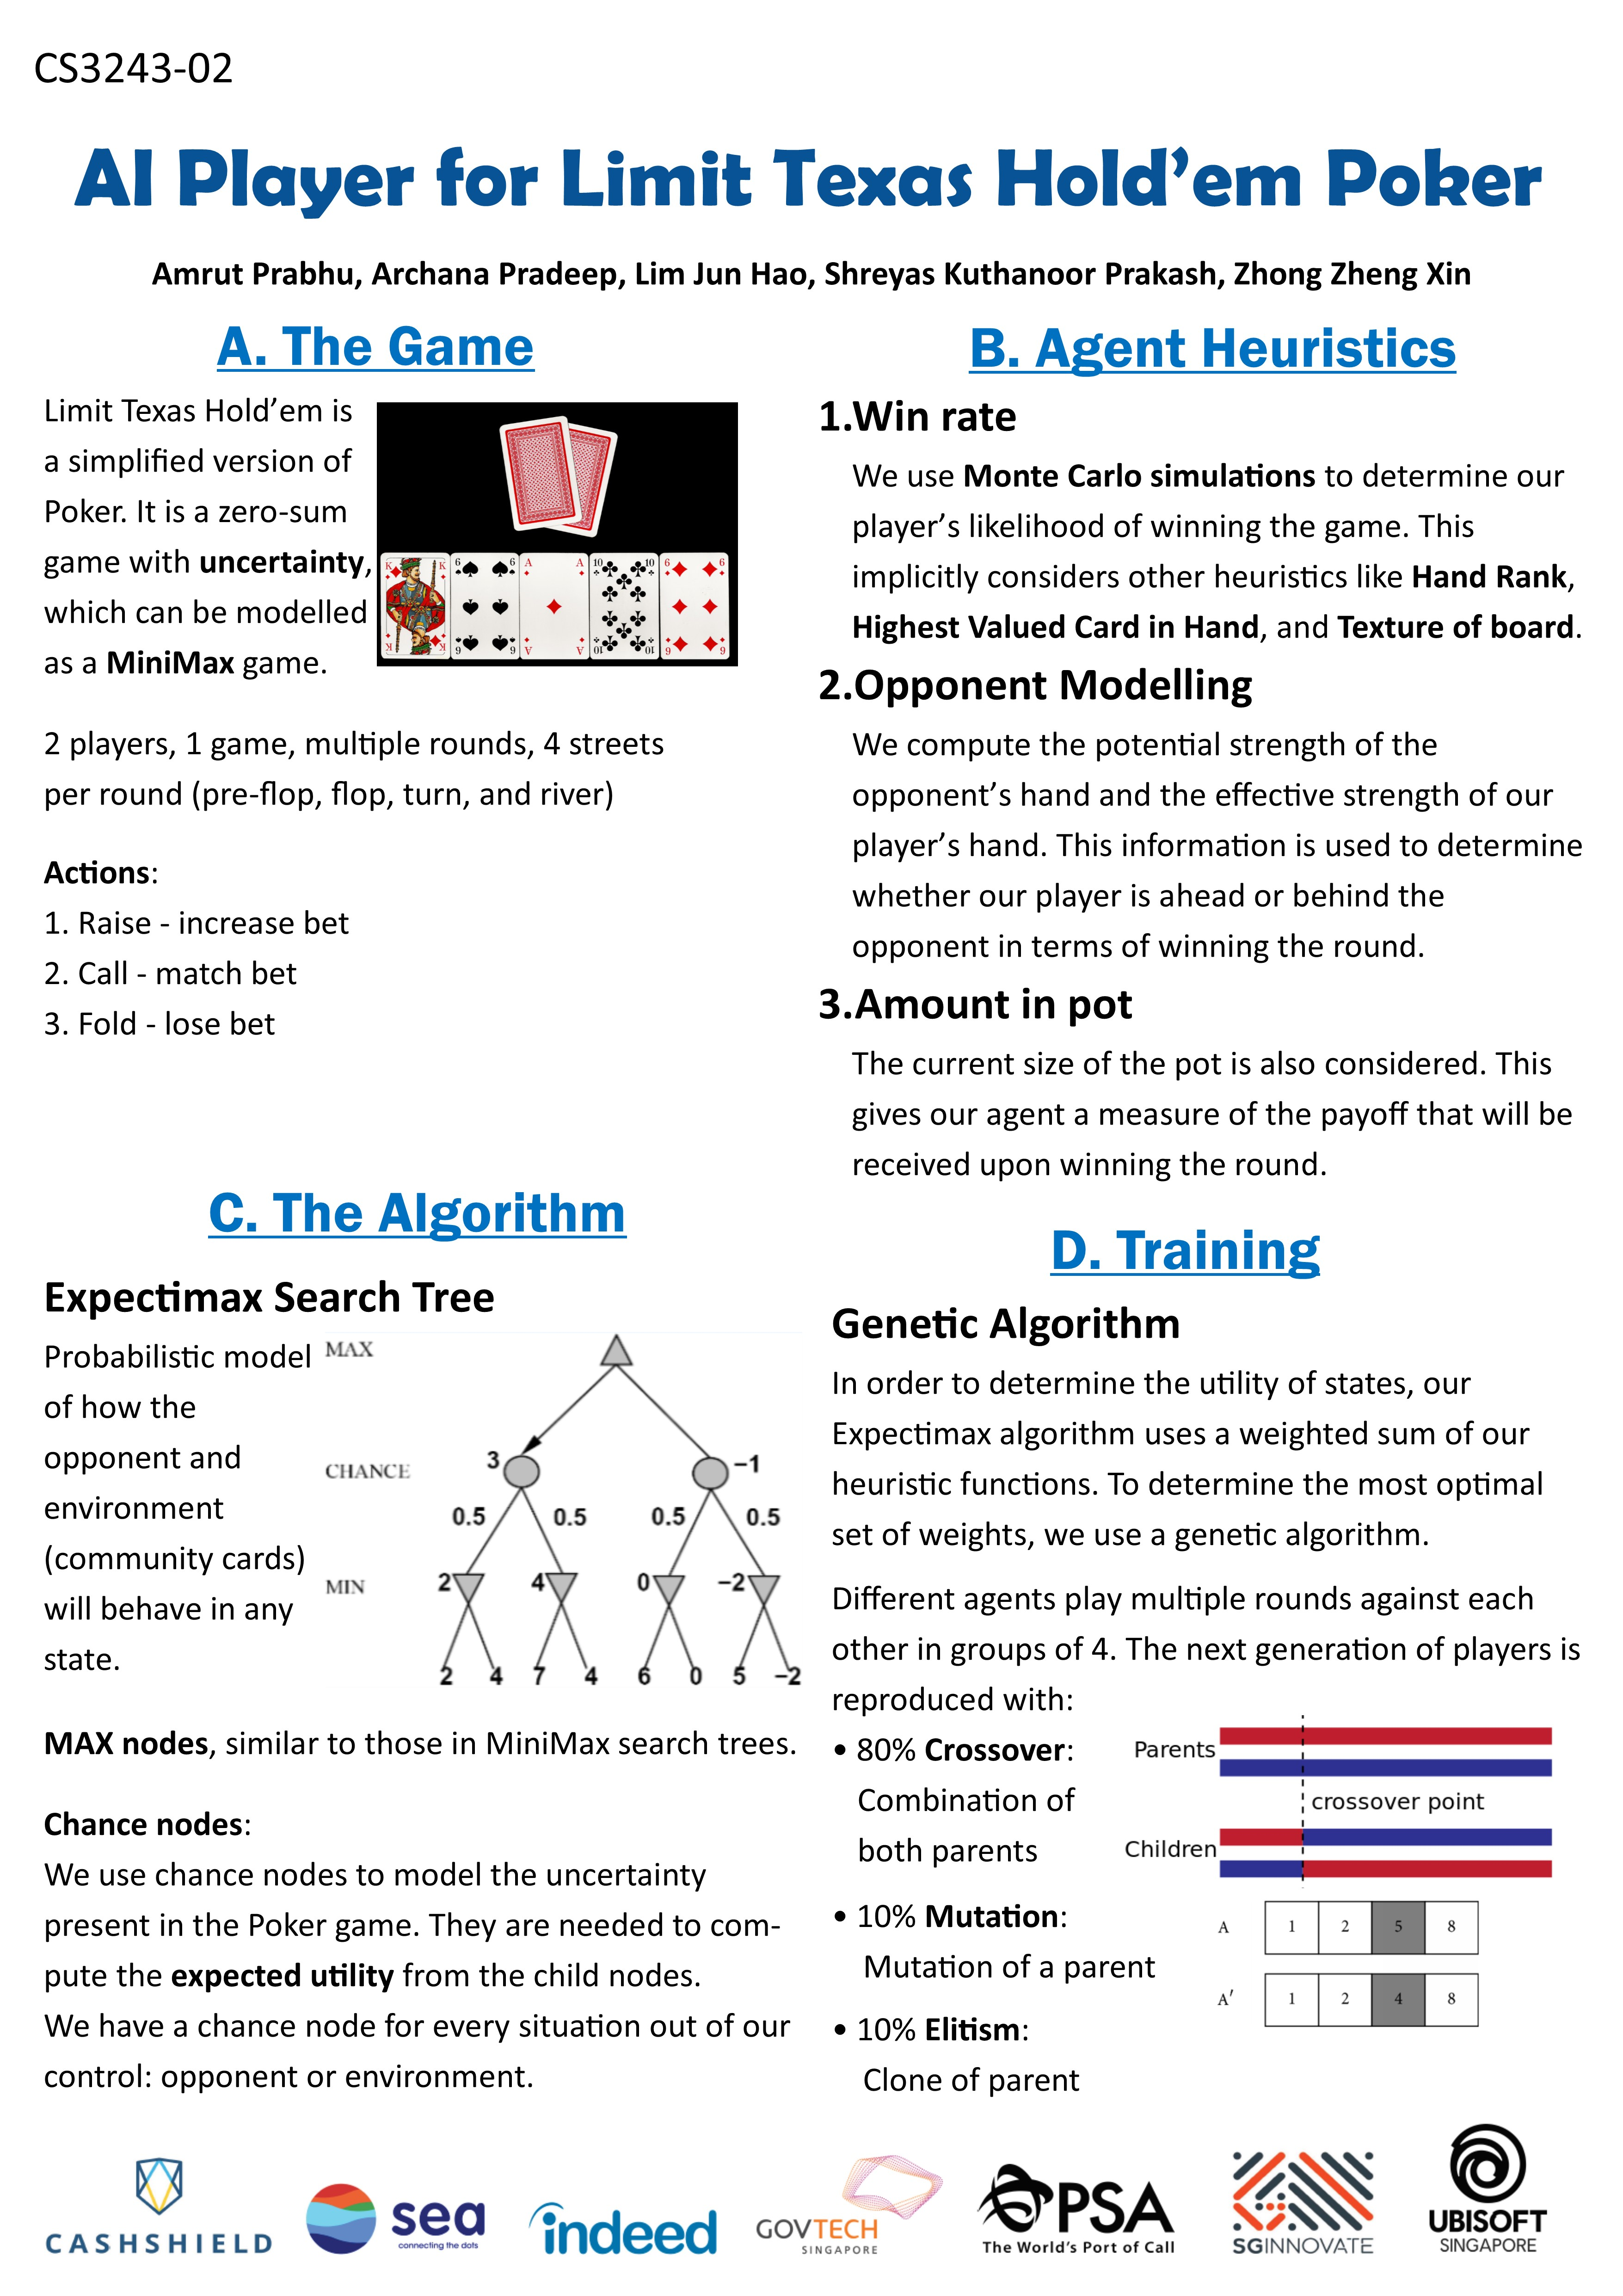
\includegraphics[width=0.5\textwidth]{test.jpg}
	\caption{\textbf{Live-cell super-resolution microscopy with NanoJ-SRRF.} sG.}
	\label{fig:TestDiagram}
\end{figure}

Finally, (Fig. \ref{fig:TestDiagram} above) complete 

Indent when starting a new paragraph, except after major headings.

\subsection{Headings and Sections}

When necessary, headings should be used to separate major sections of
your paper. (These instructions use many headings to demonstrate their
appearance; your paper should have fewer headings.). All headings should be capitalized using Title Case.

\subsubsection{Section Headings}

Print section headings in 12-point bold type in the style shown in
these instructions. Leave a blank space of approximately 10 points
above and 4 points below section headings.  Number sections with
arabic numerals.

\subsubsection{Subsection Headings}

Print subsection headings in 11-point bold type. Leave a blank space
of approximately 8 points above and 3 points below subsection
headings. Number subsections with the section number and the
subsection number (in arabic numerals) separated by a
period.

\subsubsection{Subsubsection Headings}

Print subsubsection headings in 10-point bold type. Leave a blank
space of approximately 6 points above subsubsection headings. Do not
number subsubsections.

\subsubsection{Special Sections}

You may include an unnumbered acknowledgments section, including
acknowledgments of help from colleagues.

Any appendices directly follow the text and look like sections, except
that they are numbered with capital letters instead of arabic
numerals.

The references section is headed ``References,'' printed in the same
style as a section heading but without a number. A sample list of
references is given at the end of these instructions. Use a consistent
format for references, such as that provided by Bib\TeX{}. The reference
list should not include unpublished work.

\subsection{Citations}

Citations within the text should include the author's last name and
the year of publication, for example~\cite{gottlob:nonmon}.  Append
lowercase letters to the year in cases of ambiguity.  Treat multiple
authors as in the following examples:~\cite{abelson-et-al:scheme}
or~\cite{bgf:Lixto} (for more than two authors) and
\cite{brachman-schmolze:kl-one} (for two authors).  If the author
portion of a citation is obvious, omit it, e.g.,
Nebel~\shortcite{nebel:jair-2000}.  Collapse multiple citations as
follows:~\cite{gls:hypertrees,levesque:functional-foundations}.
\nocite{abelson-et-al:scheme}
\nocite{bgf:Lixto}
\nocite{brachman-schmolze:kl-one}
\nocite{gottlob:nonmon}
\nocite{gls:hypertrees}
\nocite{levesque:functional-foundations}
\nocite{levesque:belief}
\nocite{nebel:jair-2000}

\subsection{Footnotes}

Place footnotes at the bottom of the page in a 9-point font.  Refer to
them with superscript numbers.\footnote{This is how your footnotes
should appear.} Separate them from the text by a short
line.\footnote{Note the line separating these footnotes from the
text.} Avoid footnotes as much as possible; they interrupt the flow of
the text.

\section{Illustrations}

Place all illustrations (figures, drawings, tables, and photographs)
throughout the paper at the places where they are first discussed,
rather than at the end of the paper. If placed at the bottom or top of
a page, illustrations may run across both columns.

Illustrations must be rendered electronically or scanned and placed
directly in your document. All illustrations should be in black and
white, as color illustrations may cause problems. Line weights should
be 1/2-point or thicker. Avoid screens and superimposing type on
patterns as these effects may not reproduce well.

Number illustrations sequentially. Use references of the following
form: Figure 1, Table 2, etc. Place illustration numbers and captions
under illustrations. Leave a margin of 1/4-inch around the area
covered by the illustration and caption.  Use 9-point type for
captions, labels, and other text in illustrations.

\section*{Acknowledgments}

The preparation of these instructions and the \LaTeX{} and Bib\TeX{}
files that implement them was supported by Schlumberger Palo Alto
Research, AT\&T Bell Laboratories, and Morgan Kaufmann Publishers.
Preparation of the Microsoft Word file was supported by IJCAI.  An
early version of this document was created by Shirley Jowell and Peter
F. Patel-Schneider.  It was subsequently modified by Jennifer
Ballentine and Thomas Dean, Bernhard Nebel, and Daniel Pagenstecher.
These instructions are the same as the ones for IJCAI--05, prepared by
Kurt Steinkraus, Massachusetts Institute of Technology, Computer
Science and Artificial Intelligence Lab.

\appendix

\section{\LaTeX{} and Word Style Files}\label{stylefiles}

The \LaTeX{} and Word style files are available on the IJCAI--18
website, {\tt http://www.ijcai-18.org/}.
These style files implement the formatting instructions in this
document.

The \LaTeX{} files are {\tt ijcai18.sty} and {\tt ijcai18.tex}, and
the Bib\TeX{} files are {\tt named.bst} and {\tt ijcai18.bib}. The
\LaTeX{} style file is for version 2e of \LaTeX{}, and the Bib\TeX{}
style file is for version 0.99c of Bib\TeX{} ({\em not} version
0.98i). The {\tt ijcai18.sty} file is the same as the {\tt
ijcai07.sty} file used for IJCAI--07.

The Microsoft Word style file consists of a single file, {\tt
ijcai18.doc}. This template is the same as the one used for
IJCAI--07.

These Microsoft Word and \LaTeX{} files contain the source of the
present document and may serve as a formatting sample.  


%% The file named.bst is a bibliography style file for BibTeX 0.99c
\bibliographystyle{named}
\bibliography{ijcai18}

\end{document}

